\documentclass[11pt,a4paper]{article}

\usepackage[margin=1in]{geometry}
\usepackage[T1]{fontenc}
\usepackage{lmodern}
\usepackage{microtype}
\usepackage{graphicx}
\usepackage{xcolor}
\usepackage{hyperref}
\usepackage{enumitem}
\usepackage{titlesec}
\usepackage{tikz}
\usepackage{listings}
\usepackage{booktabs}
\usepackage{fancyhdr}
\usepackage{longtable}
\usetikzlibrary{arrows.meta,positioning,shapes.geometric,fit,backgrounds,calc}

\definecolor{primary}{HTML}{1F4E79}
\definecolor{accent}{HTML}{C00000}
\definecolor{muted}{HTML}{595959}
\definecolor{codebg}{HTML}{F5F5F5}
\definecolor{codekw}{HTML}{0B5FA5}
\definecolor{codestr}{HTML}{008000}
\definecolor{codecom}{HTML}{808080}

\hypersetup{colorlinks=true,linkcolor=primary,urlcolor=primary,citecolor=primary}

\titleformat{\section}{\Large\bfseries\color{primary}}{\thesection}{1em}{}
\titleformat{\subsection}{\large\bfseries\color{primary}}{\thesubsection}{1em}{}
\titleformat{\subsubsection}{\normalsize\bfseries\color{muted}}{\thesubsubsection}{1em}{}

\pagestyle{fancy}
\fancyhf{}
\fancyhead[L]{\textit{Atlas: A Linearizable Sharded KV Store}}
\fancyhead[R]{\textit{Technical Specification}}
\fancyfoot[C]{\thepage}

\lstdefinestyle{gostyle}{
  backgroundcolor=\color{codebg},
  basicstyle=\ttfamily\small,
  keywordstyle=\color{codekw}\bfseries,
  stringstyle=\color{codestr},
  commentstyle=\color{codecom}\itshape,
  breaklines=true,showstringspaces=false,
  frame=single,framerule=0pt,
  xleftmargin=0.5em,xrightmargin=0.5em,
  aboveskip=0.8em,belowskip=0.8em,
  language=Go
}
\lstset{style=gostyle}

\title{
  \vspace{-2em}
  {\color{primary}\Huge\textbf{Atlas}}\\[0.3em]
  {\Large A Linearizable, Raft-Backed, Sharded Key-Value Store}\\[0.5em]
  {\normalsize\color{muted}\textit{Technical Specification \& Architecture Document}}
}
\author{Sithumli Nanayakkara}
\date{\today}

\begin{document}

\maketitle
\thispagestyle{fancy}
\vspace{-1em}

\begin{abstract}
\noindent
\textbf{Atlas} is a fault-tolerant, horizontally-scalable key-value store written in Go. It provides \textit{linearizable} reads and writes across a cluster of replicated shard groups, coordinated by a Raft-based configuration service. The system withstands minority node failures, network partitions, and live shard rebalancing without dropping client requests. Atlas is designed from first principles as a teaching-grade-but-production-shaped system inspired by MIT 6.824, Google Spanner's directory-based sharding model, and the ideas introduced in the Raft consensus paper by Ongaro and Ousterhout (2014). This document defines the goals, non-goals, architecture, feature set, implementation milestones, and verification strategy for the system.
\end{abstract}

\vspace{0.5em}
\hrule
\vspace{1em}

\tableofcontents
\newpage

\section{Motivation}

Distributed systems form the substrate of every modern cloud platform. The three core problems---\textit{replication}, \textit{consistency}, and \textit{partitioning}---are almost universally solved via some combination of consensus algorithms, strong consistency models, and sharding. Yet most students graduate having only \textit{used} these systems rather than built them.

Atlas is an end-to-end implementation that forces engagement with every non-trivial concern in the space:

\begin{itemize}[leftmargin=1.5em,itemsep=0.2em]
  \item How does a cluster elect a leader when messages are dropped, reordered, or delayed?
  \item How do we guarantee that a committed operation is never lost, even under power failure?
  \item How does a client observe a total order of operations when replicas disagree?
  \item How do we move data between servers \textit{while the system is serving live traffic}?
  \item How do we prove correctness under adversarial conditions?
\end{itemize}

The answers require Raft for consensus, write-ahead logging for durability, linearizability as a correctness criterion, a two-phase shard migration protocol, and aggressive fault injection in testing.

\section{Goals and Non-Goals}

\subsection{Goals}
\begin{enumerate}[leftmargin=1.5em,itemsep=0.2em]
  \item \textbf{Linearizability.} Every completed client operation appears to occur atomically at some instant between invocation and response.
  \item \textbf{Fault tolerance.} Tolerate $f$ failures out of $2f+1$ replicas per group.
  \item \textbf{Horizontal scalability.} Throughput scales approximately linearly with the number of replica groups.
  \item \textbf{Live reconfiguration.} Shards may be added, removed, or rebalanced with zero downtime.
  \item \textbf{Crash recovery.} Any node may restart at any time and rejoin without human intervention.
  \item \textbf{Verifiable correctness.} Pass automated linearizability checks under adversarial conditions.
\end{enumerate}

\subsection{Non-Goals}
\begin{enumerate}[leftmargin=1.5em,itemsep=0.2em]
  \item \textbf{Cross-shard transactions.} Per-key linearizability only in v1.
  \item \textbf{Byzantine fault tolerance.} Crash-stop failure model only.
  \item \textbf{Production-grade ops tooling.} No web UI, RBAC, or multi-tenant quotas.
  \item \textbf{Geo-replication.} Single-datacenter deployment.
\end{enumerate}

\section{Tech Stack}

\begin{longtable}{@{}p{3.2cm}p{4cm}p{7.5cm}@{}}
\toprule
\textbf{Layer} & \textbf{Technology} & \textbf{Rationale} \\
\midrule
\endhead
Language & Go 1.22+ & Goroutines map cleanly to Raft's concurrent agents; \texttt{-race} catches bugs early. \\
\addlinespace
RPC & custom in-memory\newline \texttt{google.golang.org/grpc} & Deterministic fault-injectable transport for tests; gRPC for external interfaces. \\
\addlinespace
Serialisation & \texttt{encoding/gob}\newline Protocol Buffers & Gob for internal log entries; protobuf for wire format. \\
\addlinespace
Persistence & Custom file persister\newline BoltDB / Pebble (v2) & Simple file-based persister in v1; LSM engine for larger workloads later. \\
\addlinespace
Testing & \texttt{go test -race}\newline Porcupine & Race detector in CI; linearizability checking on every commit. \\
\addlinespace
Observability & OpenTelemetry\newline Prometheus, Grafana & Tracing + metrics for leader elections, commit latency, migrations. \\
\addlinespace
Build \& CI & Go modules, GitHub Actions, golangci-lint & Reproducible builds; CI matrix covers race + Porcupine. \\
\addlinespace
Deployment & Docker, docker-compose\newline Kubernetes (stretch) & Local multi-node clusters; K8s StatefulSet as stretch goal. \\
\bottomrule
\end{longtable}

\section{System Architecture}

Atlas has four logical tiers:

\begin{enumerate}[leftmargin=1.5em,itemsep=0.2em]
  \item \textbf{Client library} — routes requests based on shard-to-group mapping.
  \item \textbf{Shard Controller} — Raft-replicated service owning the authoritative configuration.
  \item \textbf{Replica Groups} — 3- or 5-node Raft clusters serving a subset of shards.
  \item \textbf{Raft core} — reusable library used by both the controller and the replica groups.
\end{enumerate}

\begin{figure}[h!]
\centering
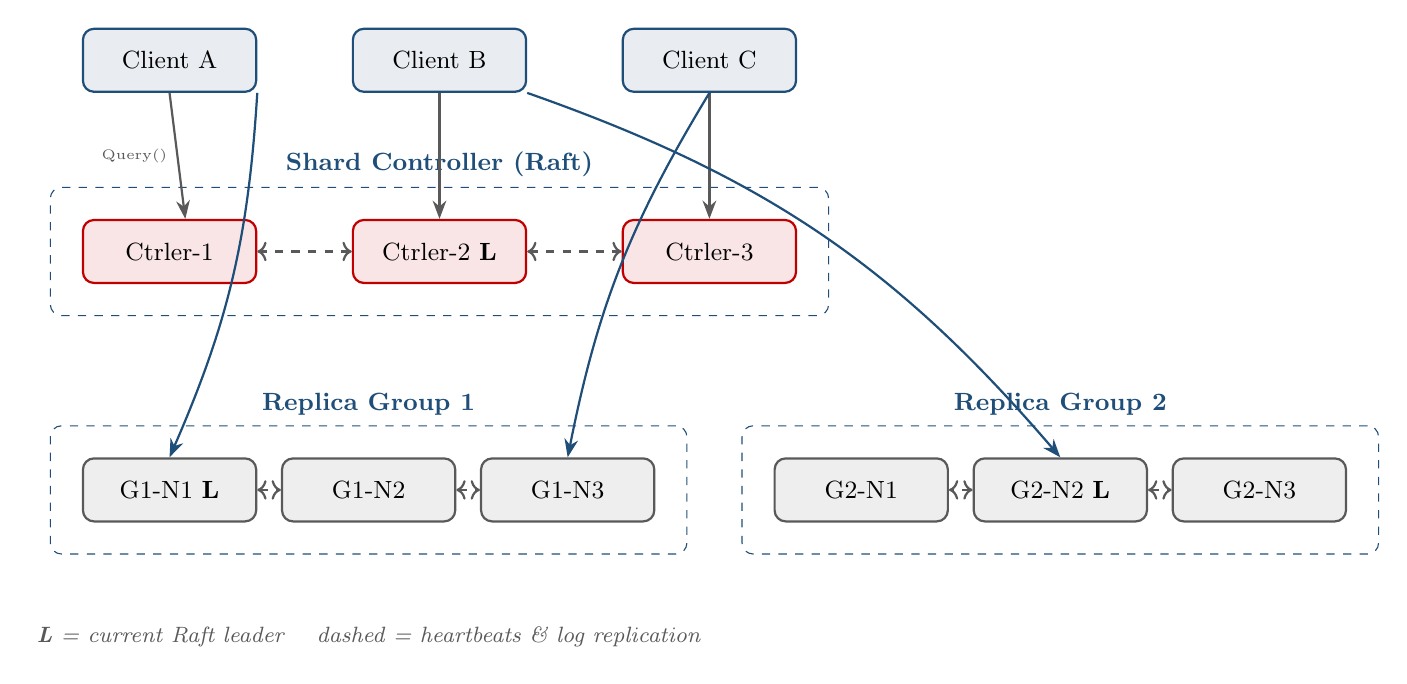
\begin{tikzpicture}[
  node distance=0.7cm and 1.2cm,every node/.style={font=\small},
  client/.style={rectangle, rounded corners, draw=primary, thick, fill=primary!10, minimum width=2.2cm, minimum height=0.8cm},
  ctrl/.style={rectangle, rounded corners, draw=accent, thick, fill=accent!10, minimum width=2.2cm, minimum height=0.8cm},
  replica/.style={rectangle, rounded corners, draw=muted, thick, fill=muted!10, minimum width=2.2cm, minimum height=0.8cm},
  group/.style={rectangle, rounded corners, dashed, draw=primary, inner sep=0.4cm},
  arrow/.style={-Stealth, thick, muted}
]
\node[client] (c1) {Client A};
\node[client, right=of c1] (c2) {Client B};
\node[client, right=of c2] (c3) {Client C};

\node[ctrl, below=1.6cm of c1] (sc1) {Ctrler-1};
\node[ctrl, right=of sc1] (sc2) {Ctrler-2 \textbf{L}};
\node[ctrl, right=of sc2] (sc3) {Ctrler-3};

\node[replica, below=2.2cm of sc1] (g1a) {G1-N1 \textbf{L}};
\node[replica, right=0.3cm of g1a] (g1b) {G1-N2};
\node[replica, right=0.3cm of g1b] (g1c) {G1-N3};

\node[replica, right=1.5cm of g1c] (g2a) {G2-N1};
\node[replica, right=0.3cm of g2a] (g2b) {G2-N2 \textbf{L}};
\node[replica, right=0.3cm of g2b] (g2c) {G2-N3};

\begin{pgfonlayer}{background}
  \node[group, fit=(sc1)(sc2)(sc3), label={[primary]above:\textbf{Shard Controller (Raft)}}] {};
  \node[group, fit=(g1a)(g1b)(g1c), label={[primary]above:\textbf{Replica Group 1}}] {};
  \node[group, fit=(g2a)(g2b)(g2c), label={[primary]above:\textbf{Replica Group 2}}] {};
\end{pgfonlayer}

\draw[arrow] (c1.south) -- ($(sc1.north)+(0.2,0)$) node[midway, left, font=\tiny] {Query()};
\draw[arrow] (c2.south) -- (sc2.north);
\draw[arrow] (c3.south) -- (sc3.north);

\draw[arrow, primary] (c1.south east) to[bend left=10] (g1a.north);
\draw[arrow, primary] (c2.south east) to[bend left=15] (g2b.north);
\draw[arrow, primary] (c3.south) to[bend right=10] (g1c.north);

\draw[<->, thick, muted, dashed] (sc2) -- (sc1);
\draw[<->, thick, muted, dashed] (sc2) -- (sc3);
\draw[<->, thick, muted, dashed] (g1a) -- (g1b);
\draw[<->, thick, muted, dashed] (g1b) -- (g1c);
\draw[<->, thick, muted, dashed] (g2b) -- (g2a);
\draw[<->, thick, muted, dashed] (g2b) -- (g2c);

\node[below=1.2cm of g1b, font=\footnotesize\itshape, muted] {\textbf{L} = current Raft leader \quad dashed = heartbeats \& log replication};
\end{tikzpicture}
\caption{Atlas cluster: clients, shard controller (3-node Raft), and two replica groups (3-node Raft each).}
\end{figure}

\section{Request Lifecycle}

A client \texttt{Get(k)} or \texttt{Put(k, v)} proceeds as follows:

\begin{enumerate}[leftmargin=1.5em,itemsep=0.2em]
  \item Client computes $s = \text{hash}(k) \bmod N_{\text{shards}}$.
  \item Client consults cached config for group $g$ owning shard $s$; queries controller if missing.
  \item Client sends RPC to last-known leader of $g$. On \texttt{WrongLeader}, retries next member.
  \item Leader appends op to Raft log; blocks until committed and applied to state machine.
  \item On \texttt{WrongGroup}, client refreshes config and retries.
  \item On success, client records value and \texttt{RequestId} for dedup on retries.
\end{enumerate}

\section{Feature Breakdown}

\subsection{Raft Core}

\subsubsection{Leader Election}
Randomised election timeouts in $[150, 300]$\,ms; monotonic terms; \texttt{RequestVote} RPCs grant at most one vote per term with up-to-date-log check; split-vote re-elections.

\subsubsection{Log Replication}
\texttt{AppendEntries} with \texttt{prevLogIndex}/\texttt{prevLogTerm} consistency checks; commit only when replicated to a majority \textit{and} from the current term; fast-backtrack optimisation on conflict to skip many entries per round trip.

\subsubsection{Persistence}
\texttt{currentTerm}, \texttt{votedFor}, and the log are \texttt{fsync}'d before any RPC reply that depends on them.

\subsubsection{Snapshots}
Triggered when state size exceeds threshold; log prefix discarded; laggards caught up via \texttt{InstallSnapshot}.

\subsection{KV State Machine}

\begin{itemize}[leftmargin=1.5em,itemsep=0.15em]
  \item Operations: \texttt{Get}, \texttt{Put}, \texttt{Append}.
  \item Linearizable reads via no-op log entry.
  \item Exactly-once via \texttt{(ClientId, RequestId)} dedup table.
  \item Stale-leader protection: partitioned leader's reads cannot commit.
\end{itemize}

\subsection{Sharding}

Keyspace partitioned into \texttt{NShards} (default 10). Mapping lives in a \texttt{Config} struct with monotonic \texttt{Num}. New configs produced on \texttt{Join}/\texttt{Leave}/\texttt{Move}. Rebalancer minimises shard movement.

\subsection{Shard Controller}

Raft-replicated. RPCs: \texttt{Join(gid, servers)}, \texttt{Leave(gid)}, \texttt{Move(shard, gid)}, \texttt{Query(num)}.

\subsection{Live Shard Migration}

\begin{enumerate}[leftmargin=1.5em,itemsep=0.2em]
  \item Each group polls controller for new configs.
  \item On observing $C_{n+1}$, computes shards to send/receive.
  \item Affected shards stop serving; clients see \texttt{NotReady}.
  \item Receivers pull shard state (+ per-client dedup table) from previous owner.
  \item Migration logged through Raft on both sides for durability.
  \item Configs processed in order; $C_{n+2}$ never applied before $C_{n+1}$ finishes.
\end{enumerate}

\section{Consistency Guarantees}

Atlas provides \textbf{linearizability per key}, including across reconfiguration. Cross-key operations are not serialised --- a client writing to two keys in different shards has no atomicity guarantee across them. This is the deliberate v1 simplification distinguishing Atlas from Spanner.

\section{Testing and Verification}

\subsection{Concurrency}
\texttt{go test -race} in CI on every commit.

\subsection{Fault Injection}
Internal RPC layer supports deterministic drops, delays, partitions, reorderings, and crashes driven from test code.

\subsection{Linearizability}
Client histories fed to \href{https://github.com/anishathalye/porcupine}{Porcupine}; counterexamples printed on violation.

\subsection{Chaos Matrix}
Nightly test matrix: replicas per group $\{3,5\}$, groups $\{1,3,5\}$, shards $\{1,10,100\}$, networks $\{$clean, lossy, partitioned$\}$, restarts $\{$none, periodic, adversarial$\}$, config churn $\{$quiescent, frequent$\}$.

\subsection{Benchmarks}
YCSB workloads A--F; head-to-head against etcd and CockroachDB on identical hardware.

\section{Observability}

Prometheus metrics: \texttt{atlas\_raft\_term\_total}, \texttt{atlas\_raft\_leader\_changes\_total}, \texttt{atlas\_raft\_commit\_latency\_seconds}, \texttt{atlas\_kv\_ops\_total}, \texttt{atlas\_shard\_migration\_duration\_seconds}. OpenTelemetry tracing across RPC boundaries. JSON structured logs. Pre-built Grafana dashboards.

\section{Implementation Milestones}

\begin{longtable}{@{}p{1.2cm}p{4.2cm}p{9cm}@{}}
\toprule
\textbf{Week} & \textbf{Milestone} & \textbf{Deliverable} \\
\midrule
\endhead
1--2 & Raft leader election & Nodes elect and re-elect under simulated crashes; split-vote tests pass. \\
\addlinespace
3--4 & Log replication & \texttt{AppendEntries} with consistency checks; fast-backtrack optimisation. \\
\addlinespace
5 & Persistence & State survives restarts; tests restart every node mid-operation. \\
\addlinespace
6--7 & Snapshots & \texttt{InstallSnapshot}; log truncation; laggards catch up. \\
\addlinespace
8--9 & KV state machine & Linearizable \texttt{Get}/\texttt{Put}/\texttt{Append}; Porcupine integrated. \\
\addlinespace
10 & Shard controller & Join/Leave/Move/Query; minimum-movement rebalancer. \\
\addlinespace
11--12 & Static sharding & Multiple groups serving fixed ranges; client routes correctly. \\
\addlinespace
13--14 & Live migration & Reconfig without dropping ops; clients see \texttt{NotReady} briefly. \\
\addlinespace
15 & Chaos matrix & 24-hour continuous run of full matrix passes. \\
\addlinespace
16 & Benchmarks \& writeup & YCSB results, scalability curves, GitHub README, blog post. \\
\bottomrule
\end{longtable}

\section{Stretch Goals}

\begin{enumerate}[leftmargin=1.5em,itemsep=0.2em]
  \item \textbf{ReadIndex and lease reads} (Raft thesis \S6.4).
  \item \textbf{Pre-vote} to prevent disruptive leader churn.
  \item \textbf{Joint consensus membership changes}.
  \item \textbf{Cross-shard transactions} (2PC over per-shard Raft).
  \item \textbf{Pebble backend} for larger-than-memory workloads.
  \item \textbf{Jepsen test suite} with Elle checker.
  \item \textbf{Multi-datacenter mode} via flexible Paxos quorums.
\end{enumerate}

\section{References}

\begin{enumerate}[leftmargin=1.5em,itemsep=0.2em]
  \item Ongaro, D., Ousterhout, J. \textit{In Search of an Understandable Consensus Algorithm.} USENIX ATC, 2014.
  \item Ongaro, D. \textit{Consensus: Bridging Theory and Practice.} PhD thesis, Stanford, 2014.
  \item MIT 6.5840 Distributed Systems, Labs 2--4. \url{https://pdos.csail.mit.edu/6.824/}
  \item Corbett, J. C. et al. \textit{Spanner.} OSDI, 2012.
  \item Herlihy, M., Wing, J. \textit{Linearizability.} TOPLAS, 1990.
  \item Athalye, A. \textit{Porcupine.} \url{https://github.com/anishathalye/porcupine}
  \item Jepsen analyses. \url{https://jepsen.io/analyses}
\end{enumerate}

\vspace{2em}\hrule\vspace{0.5em}
\begin{center}\small\color{muted}\textit{Atlas --- Technical Specification --- Sithumli Nanayakkara}\end{center}

\end{document}
